%% abtex2-modelo-trabalho-academico.tex, v-1.9.6 laurocesar
%% Copyright 2012-2016 by abnTeX2 group at http://www.abntex.net.br/ 
%%
%% This work may be distributed and/or modified under the
%% conditions of the LaTeX Project Public License, either version 1.3
%% of this license or (at your option) any later version.
%% The latest version of this license is in
%%   http://www.latex-project.org/lppl.txt
%% and version 1.3 or later is part of all distributions of LaTeX
%% version 2005/12/01 or later.
%%
%% This work has the LPPL maintenance status `maintained'.
%% 
%% The Current Maintainer of this work is the abnTeX2 team, led
%% by Lauro César Araujo. Further information are available on 
%% http://www.abntex.net.br/
%%
%% This work consists of the files abntex2-modelo-trabalho-academico.tex,
%% abntex2-modelo-include-comandos and abntex2-modelo-references.bib
%%

% ------------------------------------------------------------------------
% ------------------------------------------------------------------------
% abnTeX2: Modelo de Trabalho Academico (tese de doutorado, dissertacao de
% mestrado e trabalhos monograficos em geral) em conformidade com 
% ABNT NBR 14724:2011: Informacao e documentacao - Trabalhos academicos -
% Apresentacao
% ------------------------------------------------------------------------
% ------------------------------------------------------------------------

\documentclass[
	% -- opções da classe memoir --
	12pt,				% tamanho da fonte
	openright,			% capítulos começam em pág ímpar (insere página vazia caso preciso)
	oneside,			% para impressão em recto e verso. Oposto a oneside
	a4paper,			% tamanho do papel. 
	% -- opções da classe abntex2 --
	%chapter=TITLE,		% títulos de capítulos convertidos em letras maiúsculas
	%section=TITLE,		% títulos de seções convertidos em letras maiúsculas
	%subsection=TITLE,	% títulos de subseções convertidos em letras maiúsculas
	%subsubsection=TITLE,% títulos de subsubseções convertidos em letras maiúsculas
	% -- opções do pacote babel --
	english,			% idioma adicional para hifenização
	%french,				% idioma adicional para hifenização
	%spanish,			% idioma adicional para hifenização
	brazil				% o último idioma é o principal do documento
	]{abntex2}

% ---
% Pacotes básicos 
% ---
\usepackage{lmodern}			% Usa a fonte Latin Modern
\usepackage{newtxtext,newtxmath}
\usepackage[T1]{fontenc}		% Selecao de codigos de fonte.
\usepackage[utf8]{inputenc}		% Codificacao do documento (conversão automática dos acentos)
\usepackage{lastpage}			% Usado pela Ficha catalográfica
\usepackage{indentfirst}		% Indenta o primeiro parágrafo de cada seção.
\usepackage{color}				% Controle das cores
\usepackage{graphicx}			% Inclusão de gráficos
\usepackage{microtype} 			% para melhorias de justificação
% ---
		
% ---
% Pacotes adicionais, usados apenas no âmbito do Modelo Canônico do abnteX2
% ---
\usepackage{lipsum}				% para geração de dummy text
% ---

% ---
% Pacotes de citações
% ---
%\usepackage[brazilian,hyperpageref]{backref}	 % Paginas com as citações na bibl
\usepackage[num,abnt-etal-list=0]{abntex2cite}	% Citações padrão ABNT
\citebrackets[]
% ---
% Personalizações relativas ao padrão estabelecido pela UNESP
% ---
\usepackage{style/dissertacao}

% ---
% Informações de dados para CAPA e FOLHA DE ROSTO
% ---
\titulo{Inserir o Título do Trabalho}
\autor{Nome do Autor}
\local{Inserir Cidade}
\data{2019}
\orientador{Prof. Dr. ...}
%\coorientador{Equipe \abnTeX}
\instituicao{%
  UNIVERSIDADE ESTADUAL PAULISTA "Júlio de Mesquita Filho" -- UNESP
}
\tipotrabalho{Dissertação (Mestrado)}
% O preambulo deve conter o tipo do trabalho, o objetivo, 
% o nome da instituição e a área de concentração 
\preambulo{Dissertação apresentada como parte dos requisitos para obtenção do
título de Mestre em Ciência da Computação, junto ao Programa de Pós-Graduação
em Ciência da Computação, do Instituto de [Inserir o Instituto] da
Universidade Estadual Paulista "Júlio de Mesquita Filho", Câmpus de [Inserir
cidade].}
% ---


% ---
% Configurações de aparência do PDF final

% alterando o aspecto da cor azul
%\definecolor{blue}{RGB}{41,5,195}

% informações do PDF
\makeatletter
\hypersetup{
    %pagebackref=true,
		pdftitle={\@title}, 
		pdfauthor={\@author},
    pdfsubject={\imprimirpreambulo},
	  pdfcreator={LaTeX with abnTeX2},
		pdfkeywords={abnt}{latex}{abntex}{abntex2}{trabalho acadêmico}, 
		colorlinks=true,       		% false: boxed links; true: colored links
    linkcolor=black,          	% color of internal links
    citecolor=black,        		% color of links to bibliography
    filecolor=black,      		% color of file links
		urlcolor=black,
		bookmarksdepth=4
}
\makeatother
% --- 

% --- 
% Espaçamentos entre linhas e parágrafos 
% --- 

% O tamanho do parágrafo é dado por:
\setlength{\parindent}{1.3cm}

% Controle do espaçamento entre um parágrafo e outro:
\setlength{\parskip}{0.2cm}  % tente também \onelineskip

% ---
% compila o indice
% ---
\makeindex
% ---

% ----
% Início do documento
% ----
\begin{document}

% Seleciona o idioma do documento (conforme pacotes do babel)
%\selectlanguage{english}
\selectlanguage{brazil}

% Retira espaço extra obsoleto entre as frases.
\frenchspacing 

% ----------------------------------------------------------
% ELEMENTOS PRÉ-TEXTUAIS
% ----------------------------------------------------------
% \pretextual

% ---
% Capa
% ---
\imprimircapa
% ---

%\frontmatter

% ---
% Folha de rosto
% (o * indica que haverá a ficha bibliográfica)
% ---
%\imprimirfolhaderosto*
\imprimirfolhaderosto
% ---

% ---
% Inserir a ficha bibliografica
% ---

% Isto é um exemplo de Ficha Catalográfica, ou ``Dados internacionais de
% catalogação-na-publicação''. Você pode utilizar este modelo como referência. 
% Porém, provavelmente a biblioteca da sua universidade lhe fornecerá um PDF
% com a ficha catalográfica definitiva após a defesa do trabalho. Quando estiver
% com o documento, salve-o como PDF no diretório do seu projeto e substitua todo
% o conteúdo de implementação deste arquivo pelo comando abaixo:
%
%\begin{fichacatalografica}
%	\includepdf{metadata/ficha_catalografica.pdf}
%\end{fichacatalografica}


% ---
% Inserir folha de aprovação
% ---

% Isto é um exemplo de Folha de aprovação, elemento obrigatório da NBR
% 14724/2011 (seção 4.2.1.3). Você pode utilizar este modelo até a aprovação
% do trabalho. Após isso, substitua todo o conteúdo deste arquivo por uma
% imagem da página assinada pela banca com o comando abaixo:
%
% \includepdf{folhadeaprovacao_final.pdf}
%
% ---

\imprimirfolhadeaprovacao

% ---
% Dedicatória
% ---
%\begin{dedicatoria}
%   \vspace*{\fill}
%   \centering
%   \noindent
%   \textit{ Este trabalho é dedicado às crianças adultas que,\\
%   quando pequenas, sonharam em se tornar cientistas.} \vspace*{\fill}
%\end{dedicatoria}
% ---

% ---
% Agradecimentos
% ---
\begin{agradecimentos}

Agradeço a ...



\end{agradecimentos}
% ---

% ---
% RESUMOS
% ---

% resumo em português
\setlength{\absparsep}{16pt} % ajusta o espaçamento dos parágrafos do resumo
\begin{resumo}

\lipsum[1 - 2]

\textbf{Palavras-chave}: lorem, ipsum, lorem ipsum.
\end{resumo}


% resumo em inglês
\begin{resumo}[Abstract]
\begin{otherlanguage*}{english}

\lipsum[3 - 4]

\textbf{Keywords}: lorem, ipsum, lorem ipsum.
\end{otherlanguage*}
\end{resumo}


% ---
% inserir lista de ilustrações
% ---
\pdfbookmark[0]{\listfigurename}{lof}
\listoffigures*
\cleardoublepage
% ---

% ---
% inserir lista de tabelas
% ---
\pdfbookmark[0]{\listtablename}{lot}
\listoftables*
\cleardoublepage
% ---

% ---
% inserir lista de abreviaturas e siglas
% ---
\begin{siglas}
  \item[API] \API
  \item[DRAM] \DRAM
  \item[HDD] \HDD
	\item[SSD] \SSD
\end{siglas}
% ---

% ---
% inserir o sumario
% ---
\pdfbookmark[0]{\contentsname}{toc}
\tableofcontents*
\cleardoublepage
% ---

% ----------------------------------------------------------
% ELEMENTOS TEXTUAIS
% ----------------------------------------------------------
\textual

% ----------------------------------------------------------
% Introdução
% ----------------------------------------------------------
%------------------------------------------------------------------------------
\chapter[Introdução]{Introdução}
\label{chap:introduction}
%------------------------------------------------------------------------------

Exemplo de uma citação \cite{HennessyPatterson2012}. Exemplo de referência de
figura: conforme pode ser observado na Figura \ref{fig:biblioteca}.

\lipsum [5 - 10]

\begin{figure}[t]
  \begin{subfigure}{.5\linewidth}
    \centering
    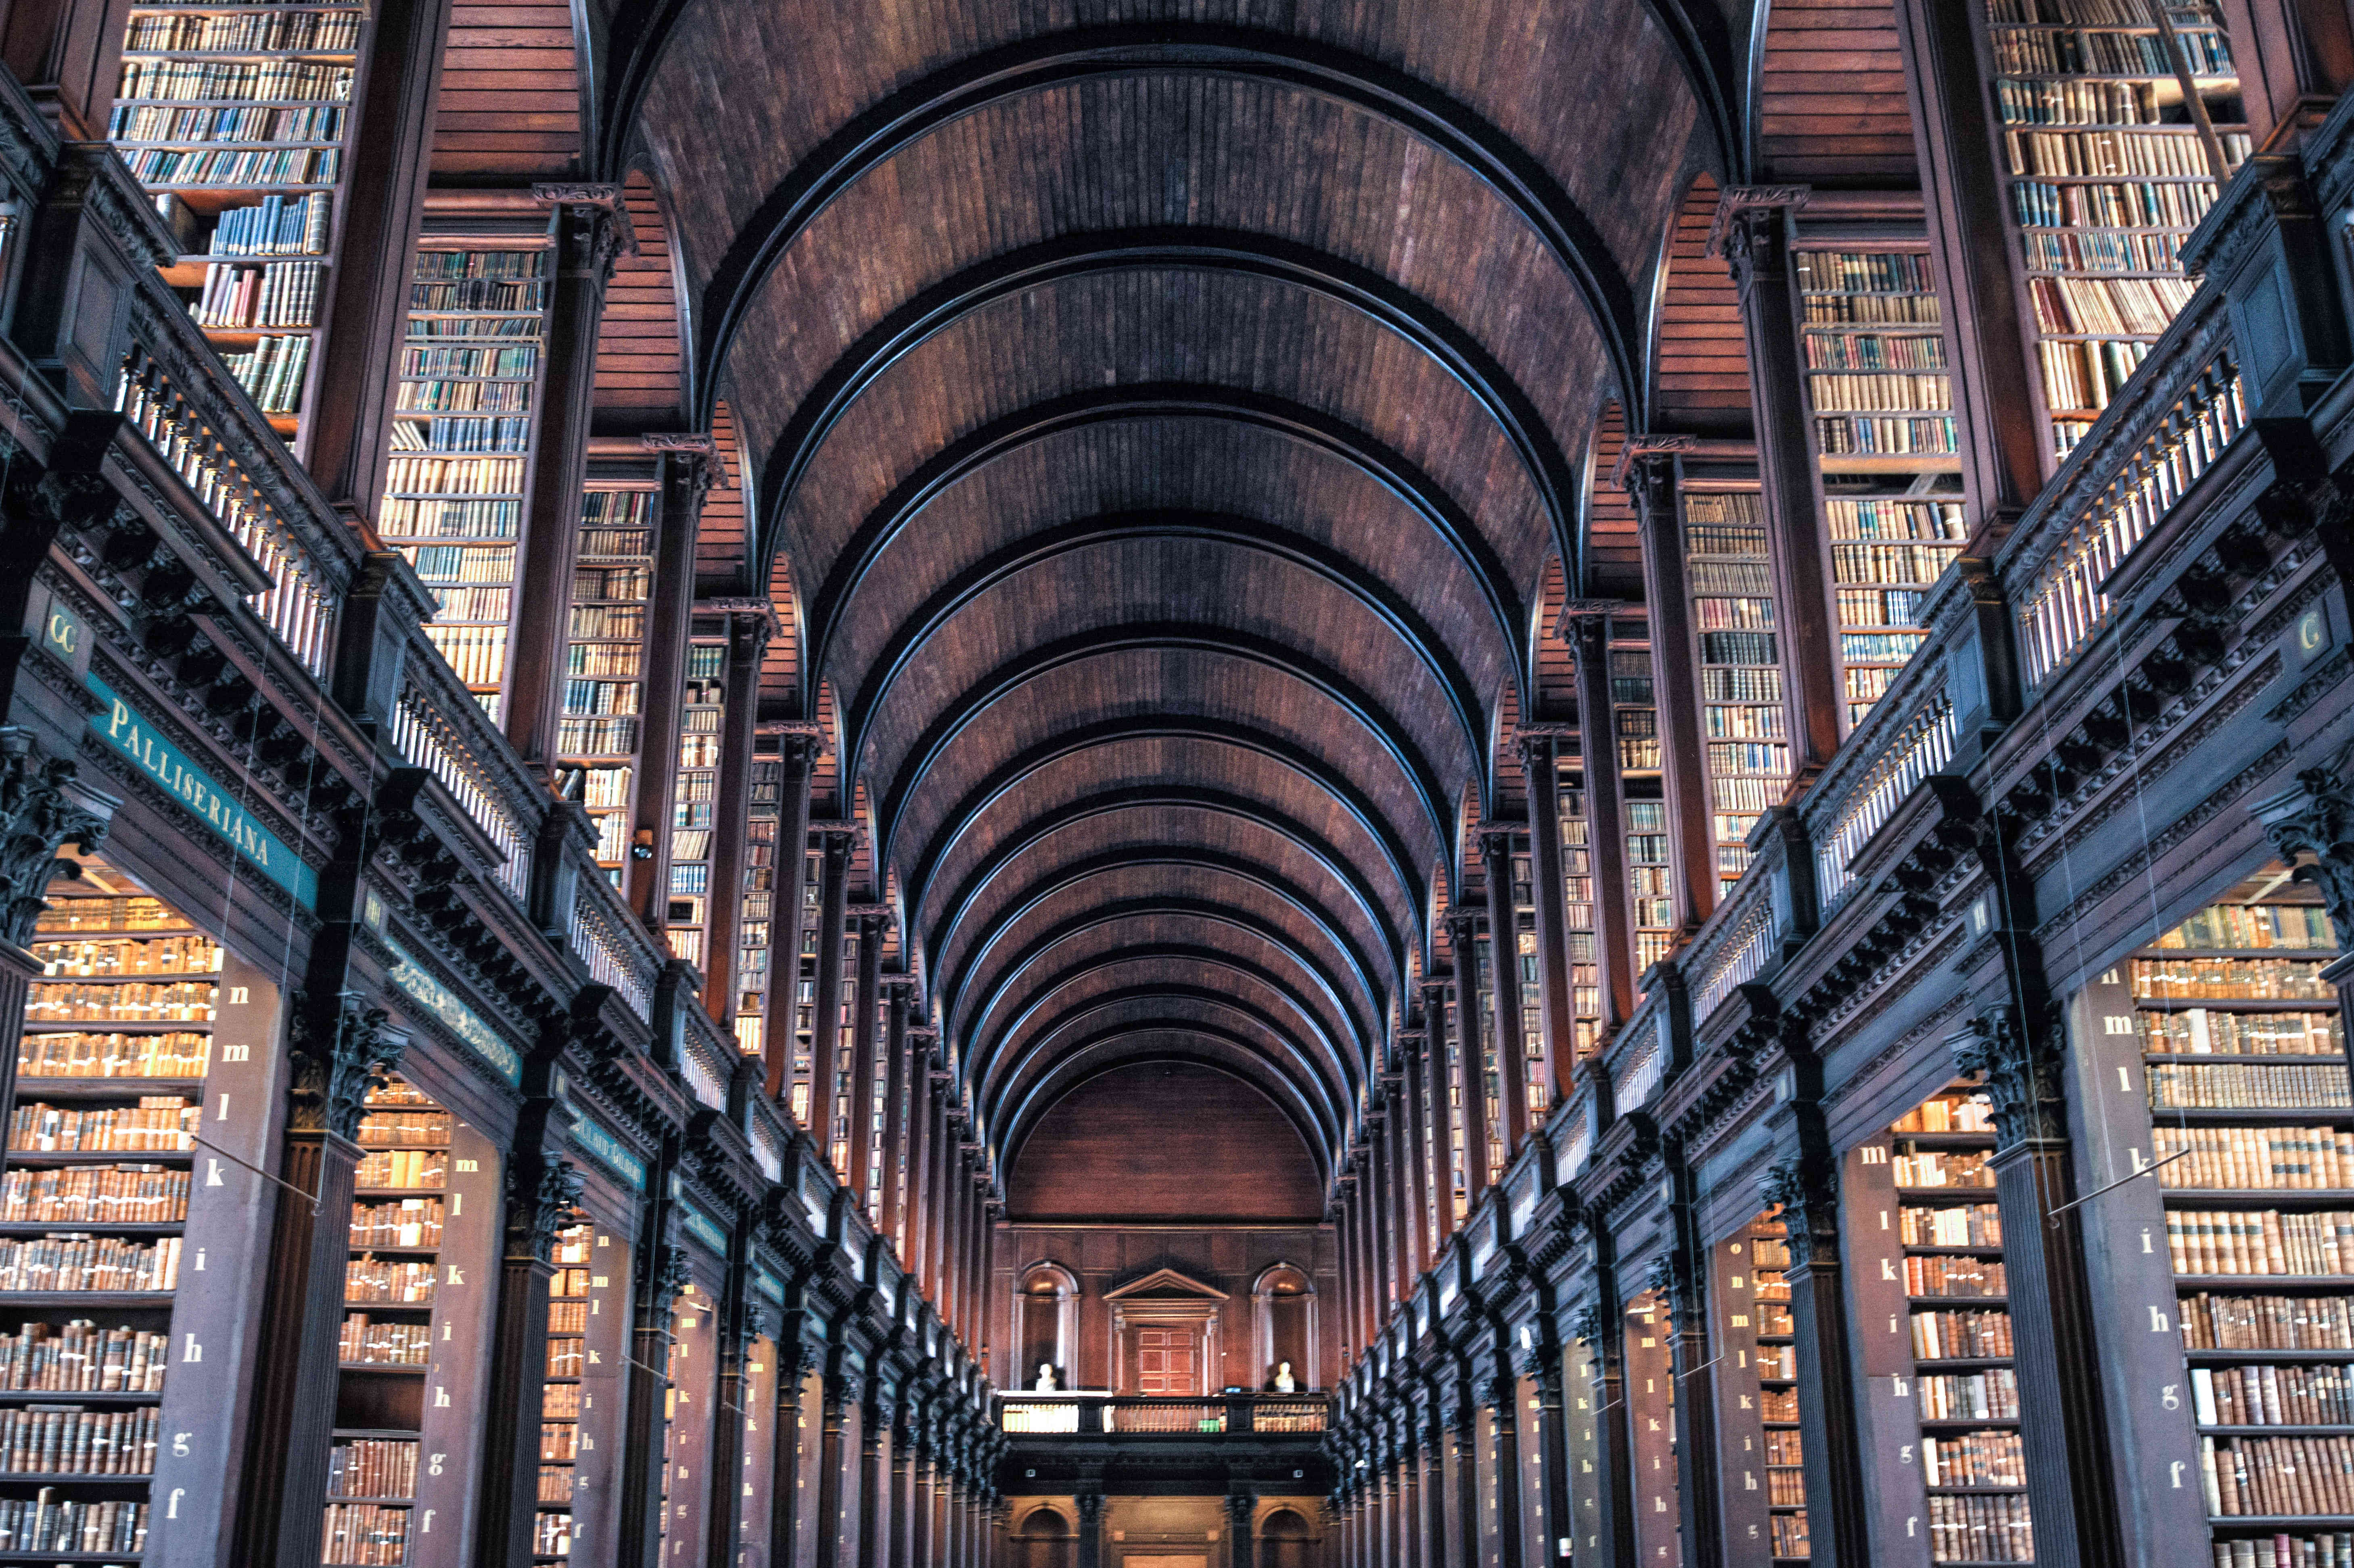
\includegraphics[width=\textwidth]{images/library1.jpg}
    \caption{Foto 1}
    \label{fig:foto1}
  \end{subfigure}
  \begin{subfigure}{.5\linewidth}
    \centering
    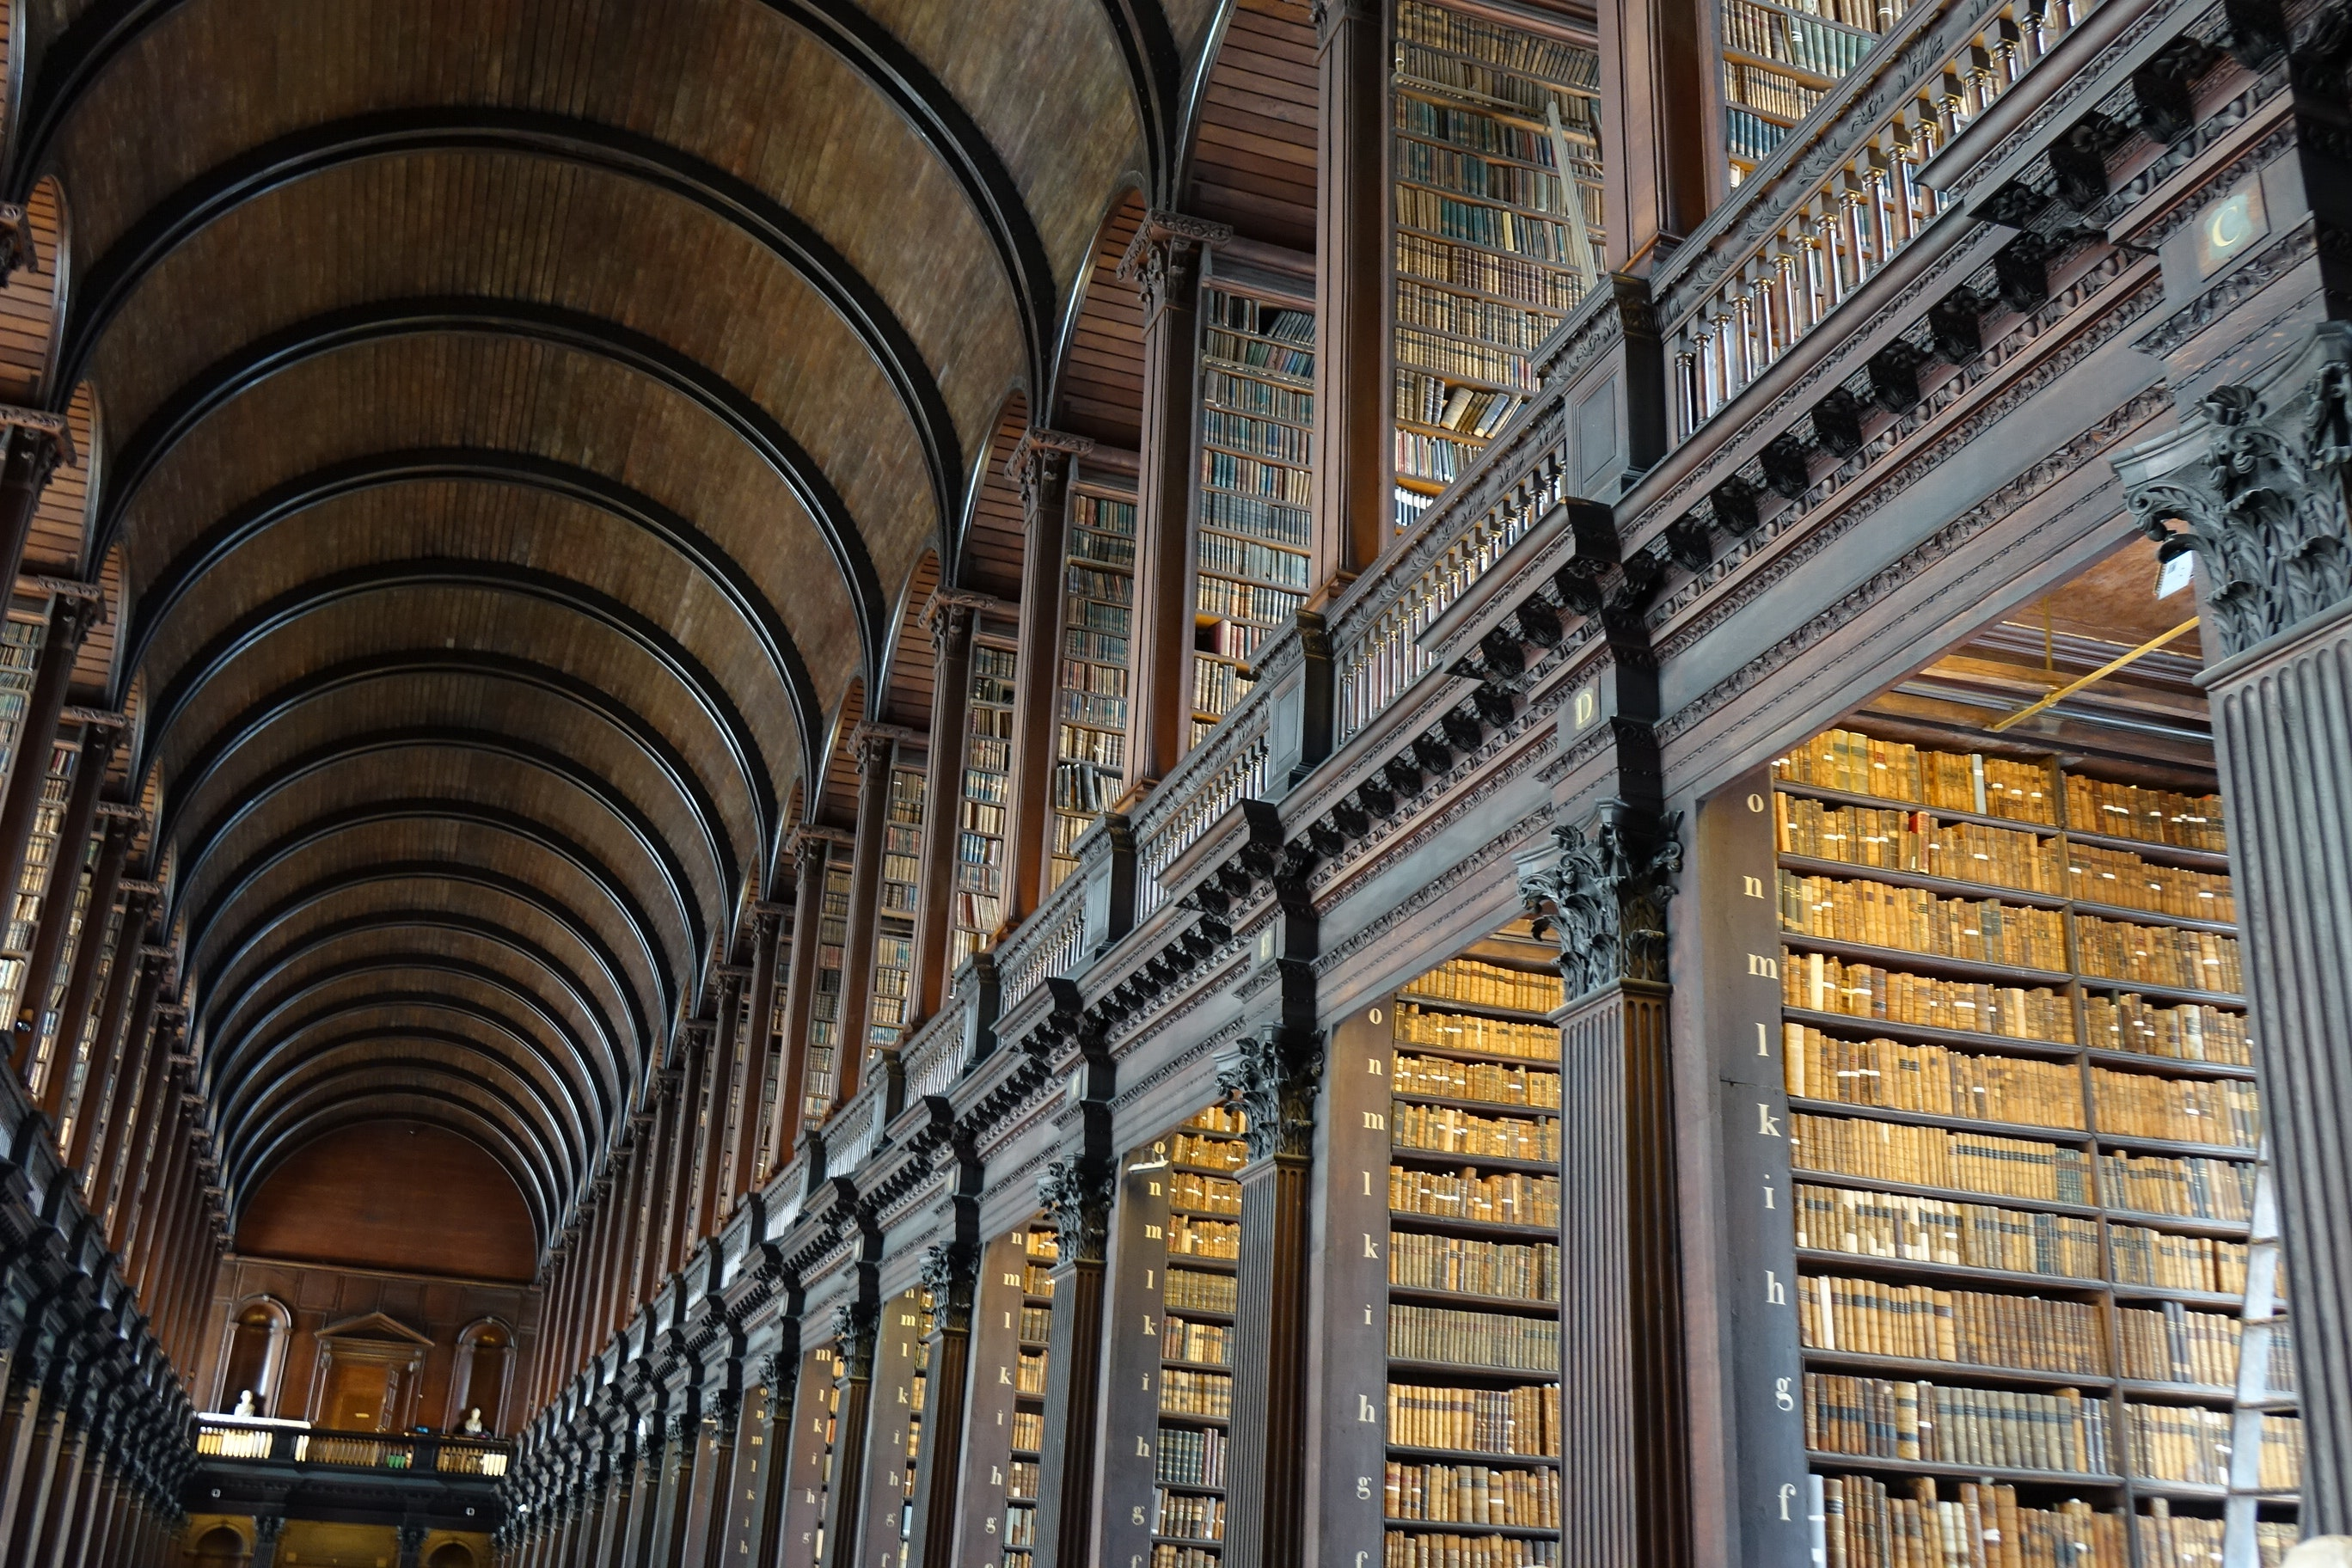
\includegraphics[width=\textwidth]{images/library2.jpg}
    \caption{Foto 2}
    \label{fig:foto2}
  \end{subfigure}
  \caption{Imagens de uma biblioteca. Extraído de ...}
  \label{fig:biblioteca}
\end{figure}


%------------------------------------------------------------------------------
\section{Objetivos e Contribuições}
\label{sec:objetivos}
%------------------------------------------------------------------------------

\lipsum[1 - 2]

%------------------------------------------------------------------------------
\section{Organização do Texto}
\label{sec:organizacao}
%------------------------------------------------------------------------------

\lipsum[3 - 3]


% ----------------------------------------------------------
% Fundamentação Teórica
% ----------------------------------------------------------
%------------------------------------------------------------------------------
\chapter[Fundamentação Teórica]{Fundamentação Teórica}
\label{chap:fundamentacao}
%------------------------------------------------------------------------------

\lipsum[4 - 6]

\begin{table}[t]
	\centering
 	\caption{Definição dos estados das linhas de cache pelo Protocolo MESI.}
 	\label{tab:mesi}
	\begin{tabular}{|l|l|}
	\hline
	\multicolumn{1}{|c|}{\textbf{Estado}} & \multicolumn{1}{c|}{\textbf{Descrição}}         \\ \hline
	Modificado 		& A linha se encontra somente na cache corrente e seu valor foi alterado  \\ \hline
	Exclusivo  		& A linha se encontra somente na cache corrente e não sofreu alterações   \\ \hline
	Compartilhado & A linha é compartilhada com as demais caches	                          \\ \hline
	Inválido      & A linha é inválida, seu valor foi alterado em alguma outra cache        \\ \hline
	\end{tabular}
\end{table}

\lipsum[7 - 10]


% ----------------------------------------------------------
% Trabalhos Relacionados
% ----------------------------------------------------------
 % ----------------------------------------------------------
\chapter[Trabalhos Relacionados]{Trabalhos Relacionados}
\label{chap:trabalhosrelacionados}
% ----------------------------------------------------------

\lipsum[4 - 6]

\lstinputlisting[caption=Inserção na tabela hash. Extraído de ...., label=alg:hash]{code/hash.c}

\lipsum[7 - 11]
 

% ----------------------------------------------------------
% Solução Proposta
% ----------------------------------------------------------
% ----------------------------------------------------------
\chapter[Solução Proposta]{Solução Proposta}
\label{chap:solucaoproposta}
% ----------------------------------------------------------

\lipsum[4 - 10]


% ----------------------------------------------------------
% Avaliação Experimental
% ----------------------------------------------------------
% ----------------------------------------------------------
\chapter[Avaliação Experimental]{Avaliação Experimental}
\label{chap:experimentos}
% ----------------------------------------------------------

\lipsum[4 - 10]


% ----------------------------------------------------------
% Conclusão
% ----------------------------------------------------------
% ----------------------------------------------------------
\chapter[Conclusão]{Conclusão}
\label{chap:conclusao}
% ----------------------------------------------------------

\lipsum[1 - 3]

% ----------------------------------------------------------
\section{Trabalhos Futuros}
\label{sec:trabalhosfuturos}
% ----------------------------------------------------------

\lipsum[4 - 6]


\postextual
% ----------------------------------------------------------

% ----------------------------------------------------------
% Referências bibliográficas
% ----------------------------------------------------------
\bibliography{references}

% ----------------------------------------------------------
% Apêndices
% ----------------------------------------------------------

% ---
% Início dos apêndices
% ---
\begin{apendicesenv}

% Imprime uma página indicando o início dos apêndices
%\partapendices*

% ----------------------------------------------------------
% Apêndice A
% ----------------------------------------------------------

\chapter{Title}

\lipsum[50]

\section{Section 1}

\lipsum[20]

\subsection{Subsection 1}

\lipsum[40]


% ----------------------------------------------------------
% Apêndice B
% ----------------------------------------------------------
\chapter{Title}

\lipsum[20]

\section{Section 1}

\lipsum[60]


% ---
% Término dos apêndices
% ---
\end{apendicesenv}

% ----------------------------------------------------------
% Anexos
% ----------------------------------------------------------

% ---
% Inicia os anexos
% ---
%\begin{anexosenv}
%
% Imprime uma página indicando o início dos anexos
%\partanexos
%
% ---
%\chapter{Morbi ultrices rutrum lorem.}
% ---
%\lipsum[30]
%
% ---
%\end{anexosenv}

%---------------------------------------------------------------------
% INDICE REMISSIVO
%---------------------------------------------------------------------
%\phantompart
%\printindex
%---------------------------------------------------------------------

%---------------------------------------------------------------------
% Permissão de Reprodução Xerográfica
%---------------------------------------------------------------------
%\includepdf{metadata/reproducao_xerografica.pdf}

\end{document}
